%----------------------------------------------------------
\usepackage{amsfonts}
\usepackage{amsmath}
%----------------------------------------------------------
\newcommand{\doclicense}{\includegraphics[width=0.09\textwidth]{doc-spec/by.eps}\xspace}%\ccShareAlike

\usepackage[T2A]{fontenc}
\usepackage[utf8]{inputenc}
% Переносы приходится выключать, т.к. при попытке прохождения нормоконтроля TestVkr будет воспринимать перенесённые слова как два слова.
%\usepackage[russian]{babel} %% это необходимо для включения переносов english
\usepackage{float}
\usepackage{rotating}
\usepackage{multirow}
\usepackage{pdflscape}
\usepackage{bm}
% необходимо для возможности копирования и поиска в готовом PDF
%\usepackage{cmap} 
\usepackage{array}
\usepackage{multicol}
\usepackage{relsize}
\usepackage{booktabs}
% Пакет необходим для поддержки многострочного подчеркивания текста
\usepackage[normalem]{ulem}
%-------------------------
% определение атрибутов сборки Git
\usepackage[grumpy, maxdepth=6]{gitinfo2}
\renewcommand{\gitMark}{[git] \textbullet{} \gitBranch\,@\,\gitAbbrevHash{} \textbullet{} \gitAuthorName, \gitAuthorEmail (\gitAuthorIsoDate)}
%-------------------------
\newcommand{\authorSID}{\Year, \group, \Author, \pdftexbanner, \jobname}
%-------------------------
%\newcommand{\authorSIDheader}[1][white]{\begin{tabular}{c}\thepage\\[-6pt]\textcolor{#1}{\tiny\authorSID}\\[-6pt]\textcolor{#1}{\tiny\gitMark}\end{tabular}}
\newcommand{\authorSIDheader}{\thepage}
%-------------------------
%\newcommand{\authorSIDright}{\begin{tabular}{c}\tiny\authorSID\\\tiny\gitMark\end{tabular}}
\newcommand{\authorSIDright}{\textcolor{gray!10.0}{\tiny\gitMark}}
%-------------------------
% Сохранение метаданных в PDF об авторе документа
\usepackage{hyperref}
\usepackage{hyperxmp}
\hypersetup{%
    pdftoolbar=true,        % show Acrobat’s toolbar?
    pdfmenubar=true,        % show Acrobat’s menu?
    pdffitwindow=false,     % window fit to page when opened
    pdfstartview={FitH},    % fits the width of the page to the window
    pdftitle={\Title},    	% title
    pdfauthor={\Author},    % author
%		pdfcopyright={Copyright © \Year, \Author. Все права защищены.},
		pdfcopyright={CC BY 4.0, \Year, \Author.},
		pdflicenseurl={http://creativecommons.org/licenses/by/4.0/},
    pdfsubject={\SubjectOfResearch},   % subject of the document
    pdfcreator={\pdftexbanner},   % creator of the document
%		pdfpublisher={Computer-aided design department, Bauman Moscow State Technical University},
		pdfcaptionwriter={Ass. Prof., PhD. Alexandr P. Sokolov},
    pdfproducer={\Author(\gitAuthorEmail), \group, \Year, Computer-aided design department, Bauman Moscow State Technical University}, % producer of the document
    pdfkeywords={\keywordsru, \keywordsen}, % producer of the document
    pdfnewwindow=true,      % links in new window
    colorlinks=true,
    citecolor=black,
    linkcolor=black,      % color of internal links (change box color with linkbordercolor)
    urlcolor=black,
    filecolor=black      % color of file links
}
%----------------------------------------------------------------
%\usepackage{xspace}
%----------------------------------------------------------
\usepackage[style=long4colheader, translate=babel, section=chapter, toc]{glossaries}
\usepackage[abbreviations, toc=true, xindy, automake]{glossaries-extra}
\setglossarystyle{treenoname}%+
\makeglossaries
%----------------------------------------------------------
% поддержка inparaenum
\usepackage{paralist} 
%----------------------------------------------------------
% нужно для определения окружения description
%\usepackage{enumitem} 
%----------------------------------------------------------------
% Настройки вставки PDF (для вставки, к примеру, направления на защиту, акта об отсутствии заимствования, рецензии)
\usepackage{pdfpages}
\includepdfset{turn=true,scale=0.95,pages=-,pagecommand={\pagestyle{fancy}}}
%----------------------------------------------------------
\usepackage{tikz}
\usetikzlibrary{tikzmark}
\usetikzlibrary{matrix,automata,graphs}
\usetikzlibrary{arrows,positioning,trees}
%----------------------------------------------------------
% необходимо для возможности включать в имена включаемых файлов _
%\usepackage[strings]{underscore}
%----------------------------------------------------------
% добавление поддержки команды вывода текста на полях \marginnote
\usepackage{marginnote}
% добавление поддержки команды \color
\usepackage{xcolor}
%--------------------------------------------
% final - удаляет все всплывающие комментарии
\usepackage[author={Alexandr Sokolov},opacity=0.1]{pdfcomment}
%\usepackage[author={Alexandr Sokolov},opacity=0.1,final]{pdfcomment}
\newcommand{\messnote}[1]{\marginnote{\color[rgb]{1,0,0}\Huge\textbf{!}\pdfcomment{#1}}[-1.0cm]}
%----------------------------------------------------------
% Произвольная нумерация списков.
\usepackage{enumerate}
%----------------------------------------------------------
%\raggedbottom
%\textwidth=163mm
%\textheight=220mm
%\oddsidemargin=-0.5pt
%\footskip=30pt
%\topmargin=27pt
%\headheight=12pt
%\headsep=25pt
%\topskip=10pt
%\baselineskip=15pt
%\topmargin=-4mm
%----------------------------------------------------------
\tolerance 1414
\hbadness 1414
\emergencystretch 1.5em
\hfuzz 0.3pt
\widowpenalty=10000
\vfuzz \hfuzz
\raggedbottom
%----------------------------------------------------------
% Настройки колонтитулов
\usepackage{fancyhdr} % Headers and footers
\fancyhf{} % clear all headers and footers - equivalent to %\fancyhead{} and \fancyfoot{}
\renewcommand{\headrulewidth}{0.0pt}
\renewcommand{\footrulewidth}{0.0pt}
%\renewcommand{\chaptermark}[1]{\markboth{ \chaptername\ \thechapter }{}} 
\renewcommand{\chaptermark}[1]{\markboth{}{}} 
\fancyhead[C]{}
\fancyfoot[C]{\authorSIDheader}%[white]}
%\setlength{\headheight}{17pt}%

\pagestyle{fancy} % All pages have headers and footers
%----------------------------------------%
%Необходимо для того, чтобы при использовании команды \thispagestyle{plain} стиль plain был переопределён на этот
\fancypagestyle{plain}{%
\fancyhf{}% clear all header and footer fields
\renewcommand{\headrulewidth}{0pt}%
\renewcommand{\footrulewidth}{0pt}%
\fancyhead[C]{}
\fancyfoot[C]{\authorSIDheader}%[white]}
}
%----------------------------------------------------------
\usepackage[hpos=0.98\paperwidth, % .98 to prevent bleed
            vpos=0.7\paperwidth,
            angle=90]{draftwatermark}

\SetWatermarkText{\authorSIDright}
%\SetWatermarkColor[gray]{0.1}
\SetWatermarkFontSize{0.2cm}
\SetWatermarkAngle{90}
\SetWatermarkHorCenter{20cm}
%----------------------------------------------------------
% указание 
\setcounter{secnumdepth}{2}
%----------------------------------------------------------
% Пакеты для подсчета количества: страниц, и т.д.
\usepackage{etoolbox}
\usepackage{totcount,assoccnt}
%----------------------------------------------------------

% суперсчетчики всего ! :-)
\regtotcounter{page}

\newtotcounter{ffigure}
\setcounter{ffigure}{0}
\def\oldfigure{} \let\oldfigure=\figure
\def\figure{\stepcounter{ffigure}\oldfigure}

\newtotcounter{ttable}
\setcounter{ttable}{0}
\def\oldtable{} \let\oldtable=\table
\def\table{\stepcounter{ttable}\oldtable}

\newtotcounter{cchapter}
\setcounter{cchapter}{0}
\def\oldchapter{} \let\oldchapter=\chapter
\def\chapter{\stepcounter{cchapter}\oldchapter}

\newtotcounter{eequation}
\setcounter{eequation}{0}
\def\oldequation{} \let\oldequation=\equation
\def\equation{\stepcounter{eequation}\oldequation}

\newtotcounter{bibcnt}
\setcounter{bibcnt}{0}
\def\oldbibitem{} \let\oldbibitem=\bibitem
\def\bibitem{\stepcounter{bibcnt}\oldbibitem}

%----------------------------------------------------------
% необходимо для работы команды \xspace (умный пробел после замены, осуществляемой некоторой командой в тексте)
\usepackage{xspace}
%----------------------------------------------------------
% необходимо для того, чтобы в окружениях enumerate можно было менять формат нумерации
%\usepackage{enumitem}
%----------------------------------------------------------
%Необходимо для сокращения размера шрифта подписей и сокращения отступов между рисунком и подписью к нему
\usepackage[margin=5pt,font={small, singlespacing}, labelfont={small}, justification=centering, labelsep=period]{caption}
\captionsetup{belowskip=0pt}
%----------------------------------------------------------
% подключение листингов и определение языков
\usepackage{listings}

\lstset
{%
		extendedchars=\true, % включаем не латиницу
		frame=tb, % рамка сверху и снизу
		escapechar=|, % |«выпадаем» в LATEX|
		xleftmargin=0.5cm,
		xrightmargin=0.5cm,
		columns=fullflexible,
%		aboveskip=5pt,
		numbers=left,                    % where to put the line-numbers; possible values are (none, left, right)
		numbersep=4pt,                   % how far the line-numbers are from the code
		showspaces=false,
		showstringspaces=false,
		breakatwhitespace=true,         % sets if automatic breaks should only happen at whitespace
		breaklines=true,                 % sets automatic line breaking
		basicstyle=\color{black}\small\sffamily,%\ttfamily,% \sffamily
		commentstyle=\color{gray}\itshape, % шрифт для комментариев
		stringstyle=\color{orange},
%		stringstyle=\bfseries, % шрифт для строк
		numberstyle=\footnotesize\color{gray},
%		numberstyle=\ttfamily\small\color{gray}, % the style that is used for the line-numbers
		keywordstyle=\color{blue}\bfseries,
%		directivestyle=\color{red},
%		emph={int,char,double,float,unsigned,bool,string},
		emphstyle={\color{blue}\bfseries},
		tabsize=2,
%		morecomment=[l]{//},
%		otherkeywords={=,==,:,&},
		texcl=true,
}

\lstloadlanguages{Python, C++}

%--------------------------------------------
% необходимо для команды \cancelto{0}{x}
\usepackage{cancel}
%----------------------------------------------------------
% необходимо для того, чтобы доопределить спецификатор P, для 
% использования в таблицах при форматировании
\usepackage{array}
\newcolumntype{P}[1]{>{\centering\arraybackslash}p{#1}}
%----------------------------------------%
% необходимо для того, чтобы допускались разрывы страниц внутри align align*
\allowdisplaybreaks
%----------------------------------------%
\makeatletter
\def\dynscriptsize{\check@mathfonts\fontsize{\sf@size}{\z@}\selectfont}
\makeatother
\def\textunderset#1#2{\leavevmode
  \vtop{\offinterlineskip\halign{%
    \hfil##\hfil\cr\strut#2\cr\noalign{\kern-.3ex}
    \hidewidth\dynscriptsize\strut#1\hidewidth\cr}}}

\newcommand\executer[1]{\textunderset{\scriptsize{подпись, дата}}{\signvrule} #1}
%----------------------------------------------------------
% необходимо для поддержки поворотов текста
\usepackage[absolute]{textpos}
\setlength{\TPHorizModule}{30mm}
\setlength{\TPVertModule}{\TPHorizModule}
\textblockorigin{0mm}{25mm} % start everything near the top-left corner
%----------------------------------------------------------
% оформление "теорем"
\usepackage{amsthm}
\usepackage{thmtools}
%----------------------------------------------------------
\newtheoremstyle{theoremstyle}% <name>
{0pt}% <Space above>
{0pt}% <Space below>
{\normalfont}% <Body font>
{0pt}% <Indent amount>
{\bfseries}% <Theorem head font>
{.}% <Punctuation after theorem head>
{.5em}% <Space after theorem headi>
{}% <Theorem head spec (can be left empty, meaning `normal')>
%----------------------------------------------------------
\theoremstyle{theoremstyle}

%\declaretheoremstyle[
  %headfont=\normalfont\bfseries,
%%	numberwithin=section,
  %bodyfont=\normalfont,
  %spaceabove=1em plus 0.75em minus 0.25em,
  %spacebelow=1em plus 0.75em minus 0.25em,
  %qed={$\blacksquare$},
	%headpunct={\newline},
%%  qed={$\square$},
%]{taskstyle}
%
%\declaretheorem[
  %style=taskstyle,
  %title=Задача,
  %refname={задача,задачи},
  %Refname={Задача,Задачи}
%]{task}
%
%\declaretheoremstyle[
  %headfont=\normalfont\bfseries,
	%numberwithin=task,
  %bodyfont=\normalfont,
  %spaceabove=1em plus 0.75em minus 0.25em,
  %spacebelow=1em plus 0.75em minus 0.25em,
	%headpunct={\newline},
%%  qed={$\blacksquare$},
  %qed={$\square$},
%]{variantstyle}
%
%\declaretheorem[
  %style=variantstyle,
  %title=Вариант,
  %refname={вариант,варианты},
  %Refname={Зариант,Варианты}
%]{variant}

%----------------------------------------------------------
%\newtheorem{question}{Вопрос}
%\newtheorem{task}{Задача}
%\newtheorem{solution}{Решение}
\newtheorem{remark}{Замечание}
\newtheorem{description}{Описание}
%%----------------------------------------------------------
